\hypertarget{_mesh_builder_8cpp}{}\section{Mesh\+Builder.\+cpp File Reference}
\label{_mesh_builder_8cpp}\index{MeshBuilder.cpp@{MeshBuilder.cpp}}


Build \mbox{\hyperlink{class_mesh}{Mesh}} Objects based on the M\+E\+S\+H\+T\+Y\+PE provided.  


{\ttfamily \#include \char`\"{}Mesh\+Builder.\+h\char`\"{}}\newline
Include dependency graph for Mesh\+Builder.\+cpp\+:
\nopagebreak
\begin{figure}[H]
\begin{center}
\leavevmode
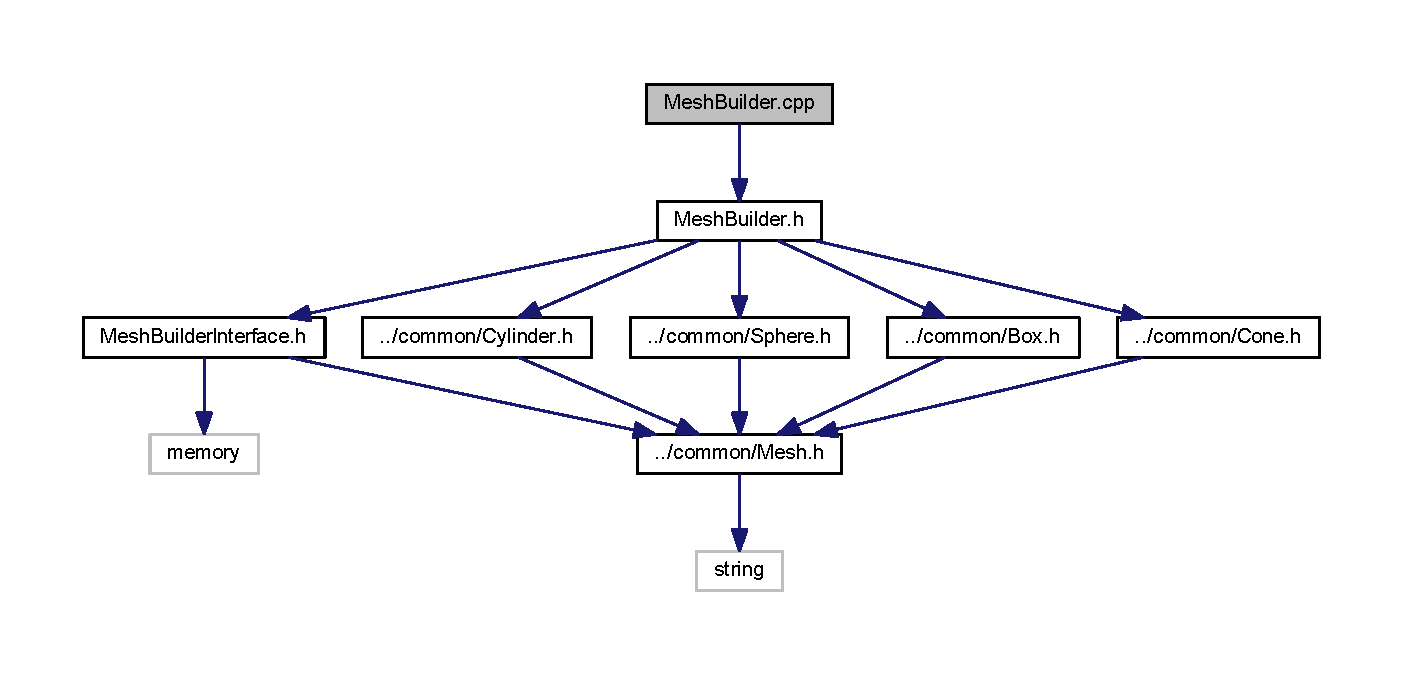
\includegraphics[width=350pt]{_mesh_builder_8cpp__incl}
\end{center}
\end{figure}


\subsection{Detailed Description}
Build \mbox{\hyperlink{class_mesh}{Mesh}} Objects based on the M\+E\+S\+H\+T\+Y\+PE provided. 

Different mesh objects are created based on the different mesh types provided \begin{DoxySeeAlso}{See also}
\mbox{\hyperlink{_mesh_builder_interface_8h_ad6436347ddb93aed826a19081b53dd61}{M\+E\+S\+H\+T\+Y\+PE}} 
\end{DoxySeeAlso}

\begin{DoxyParams}[1]{Parameters}
\mbox{\texttt{ in}}  & {\em type} & Type of mesh To generate \\
\hline
\end{DoxyParams}
\begin{DoxyReturn}{Returns}
Return the Unique pointer of the \mbox{\hyperlink{class_mesh}{Mesh}} Object 
\end{DoxyReturn}
